\documentclass{tufte-handout}
%\input{vc.tex}  % For version control
\usepackage{graphicx} 
\title{HashPipe}
\author{}
%\date{\GITAuthorDate, rev. \GITAbrHash}

\begin{document}
\maketitle
%\section{}
%\subsection

\begin{abstract}
  Implement a symbol table using a \emph{Hash Pipe} data structure.
  This exercise introduces yet another implementation of symbol tables (besides those presented in chapter 3 of [SW]) with logarithmic inseration and search.
  The main difficulty are low-level implementation choices and careful programming  similar to what is needed for implemeting a binary search tree of hash table.
\end{abstract}

\section{Description}

Write the class HashPipe that implements many of the methods for an ordered symbol table with String keys and Integer values. 
In particular, implement the following API:

\begin{quotation}
\begin{fullwidth}\small
\begin{verbatim}
public class HashPipe 

public HashPipe() // create an empty symbol table
public int size() // return the number of elements
public void put(String key, Value val) // put key-value pair into the table
public Integer get(String key) // value associated with key
public String floor(String key) // largest key less than or equal to key 
 \end{verbatim}
\end{fullwidth}
\end{quotation}

\subsection{Data structure}

The \emph{Hash Pipe} data structure is a pointer-based structure that represents every key--value pair using a so-called \emph{pipe}.
The Pipes are arranged from left to right, in sorted key order.
The entries of each pipe point to the pipes to its right, as shown here:

\begin{figure}
  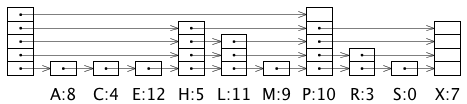
\includegraphics[width=\textwidth]{img/full.png}
  \caption{The data structure after running the basic symbol table client in [SW, 3.1] on input {\tt S E A R C H E X A M P L E}.}
\end{figure}

To be quite precise, consider key $k$.
The pipe's reference at height $h$ points to the smallest key $k'$ larger than $k$ of height at least $h$.
There is a special \emph{root} pipe to the left, which you can think of as `negative infinity.' 
The root pipe does not represent any key--value pair, no other pipe points to it, and it is at least as high as any other pipe.
References with `nothing to the left' contain \emph{null}, shown as empty boxes in the figure.

The number of entries (the `height' of a pipe) is given by the Java hash code of the key,
more specifically it is the \emph{number of trailing zeros of {\tt key.hashCode()} $+1$}.
For instance, the {\tt "A".hashCode()} is 65, which is 1000001 in binary and has no trailing zeros; thus, the height of the pipe of key ``A'' is $0+1=1$.
Similarly, the {\tt "P".hashCode()} is 80, which is 1010000 in binary and has four trailing zeros; thus, the height of the pipe of key ``P'' is $4+1=5$.

Navigation in a Hash Pipe works very much like navigation in a search tree.
To look for a key $k$, start at the root pipe on the highest level containing a reference.
Depending on the comparison with the pointed-to key $k'$, proceed either down the pipe of $k$, stay at the same level but move to the pipe of $k'$.
To insert a new key $k$, find its immediate predecessor (or `floor'), create a new pipe of the height defined by $k$, and (and this is the tricky part) update all the references.

\subsection{Deliverables}

\begin{enumerate}
\item {\tt HashPipe.java} and a report
\end{enumerate}

\subsection{Requirements}

Under the uniform hashing assumption, your update times have to be logarithmic in the number of keys.

If you use more than 100 lines of code, you are probably making a mistake.

Apart from the symbol table methods, you are required to implement a control method {\tt public String control(String key, int h)} that returns the contents of the pipe of the given {\tt key} at the given height $h$, counting from below and starting with $0$.
The control method returns the key that is referenced at that position, or \emph{null}.
For instance, in Figure 1, {\tt control("H", 3)} is ``{\tt P}'', {\tt control("H", 2)} is ``{\tt L}'', and {\tt control("P", 4)} is \emph{null}.
\footnote{This method exists partly for testing your hand-in, but it is also meant as help to you for debugging while you write your code.}

\subsection{Remarks}

\begin{enumerate}
  \item The intuition why the Hash Pipe is very fast is because the pipes have random heights.
Of course, the hash code is not random at all, and you can easily attack the performance of this data structure using maliciously chosen keys. 
A better way of deciding the height of a pipe would be to use \emph{randomness}.
(For instance, the number of consecutive `tails' in a sequence of coin flip.)
However, this is a programming exercise, and we have to be able to verify your implementation, which is why we prefer a deterministic policy for determining pipe heights.

  \item You have to write very little code, but it is \emph{very hard} to get that code right.
    You are strongly advised to use your own {\tt control} method to continuously test your constructions.
    Use pen and paper to make precise drawings for very small examples (with only 0, 1, or 2 keys in the symbol table) and use {\tt control} to make sure that all references point to where you think they do. 
    Figure 2 is your friend.

  \item The most important design decision is how you define the inner class that represents a key--value pair (you will probably call this {\tt Node} or maybe {\tt Pipe}, depending on how you do it).
      There are at least two different ways of doing this.

    \item We avoid generics in this exercise---our keys are always of type {\tt String} and our values are always of type {\tt Integer}.
      There is a reason for that\footnote{One of the ways of implementing {\tt Node} very quickly gets you bogged down into annoying details of Java's type system for generic arrays. So this restriction makes the exercise a lot easier.}, but if you are ambitious, you are welcome to write a generic symbol table with signature 
    \begin{quote}
    \tt HashPipe<Key extends Comparable<Key>, Value>
    \end{quote} 

    \item If you want, you can fix the height of the root pipe (all the way to the left) to 32 (and fill the top levels with {\emph null}).
      Otherwise, you have to rebuild the root pipe every time a new, higher, pipe enters the data structure, which involves some simple (but annoying) extra code.

  \item Hint: You will probably make your life easier by having  a private method like \begin{quote}
    \tt private Node floorNode(Key key)
    \end{quote}
    that returns the pipe of the floor of the given key.
      (The details depend a bit on how you chose to implement the pipes.)


    \item The hash pipe really shines for range queries.
      If you're ambitious (and everything else really works), implement 
      \begin{quote}
	\tt public Iterable<String> keys(String lo, String hi)
      \end{quote}
      and enjoy how easy (and fast!) that was.

    \item If you like binary arithmitic, you can count trailing zeros by repeated modulo and halving operations.
      For everybody else, there is 
    \begin{quote}
    \tt Integer.numberOfTrailingZero(int i)
  \end{quote}
  in the Java standard library.

    \item As always, follow the coding style and naming conventions in the book.

\end{enumerate}

\end{document}
